

\subsubsection{Overview}
The Instruction Planner is placed at the top layer of the whole robot fleet architecture,
therefore it is meant to be the "Swarm Manager" of all robots that work on a common task. \\
This approach is split up into two different aspects. They are shown in figure \ref{fig:instr_overview}, as the \textit{Game State Machine} and \textit{Robot State Machine}.
The \textit{Game State Machine} manages the actual state of the game (e.g. Exploration Phase) and the \textit{Robot State Machine} manages the particular state of the robots on the field (e.g. maintenance).

\subsubsection{Idea}

The following figure \ref{fig:instr_overview} shows the internal structure of the
Instruction Planner (in blue)  and how its state machines work with the overall architecture of the system (external Refbox in red and components of the robots in green).
As seen in the figure the Instruction Planner does multiple things: \newpage
In Blue (once per fleet):\\
\begin{itemize}
    \item \textbf{Game Management:}  organization of next actions
    \begin{itemize}
        \item Exploration Management
            \begin{itemize}
                \item keeps log of found machines
                \item estimates explorable positions
                \item suggests next orders to reach the objective
            \end{itemize}
        \item Production Management
        \begin{itemize}
            \item coming up
        \end{itemize}
    \end{itemize}
    \item \textbf{Fleet Management:} organization of robots and their progress
    \begin{itemize}
        \item which state they are in (e.g disqualified / maintenance / active)
        \item what they are working on
        \item error handling
    \end{itemize}
\end{itemize}

%The red and green part of figure \ref{fig:instr_overview} display the message flow of the components.
%The single Instruction Planner (deployed on one robot of the fleet) commands the Sequencers of the involved robots. The Sequencer (on each robot) coordinates the individual local components. The Sequencers send back the %detected machines to the Instruction Planner, which communicates directly with the Refbox.

\begin{figure}[h]
\centering
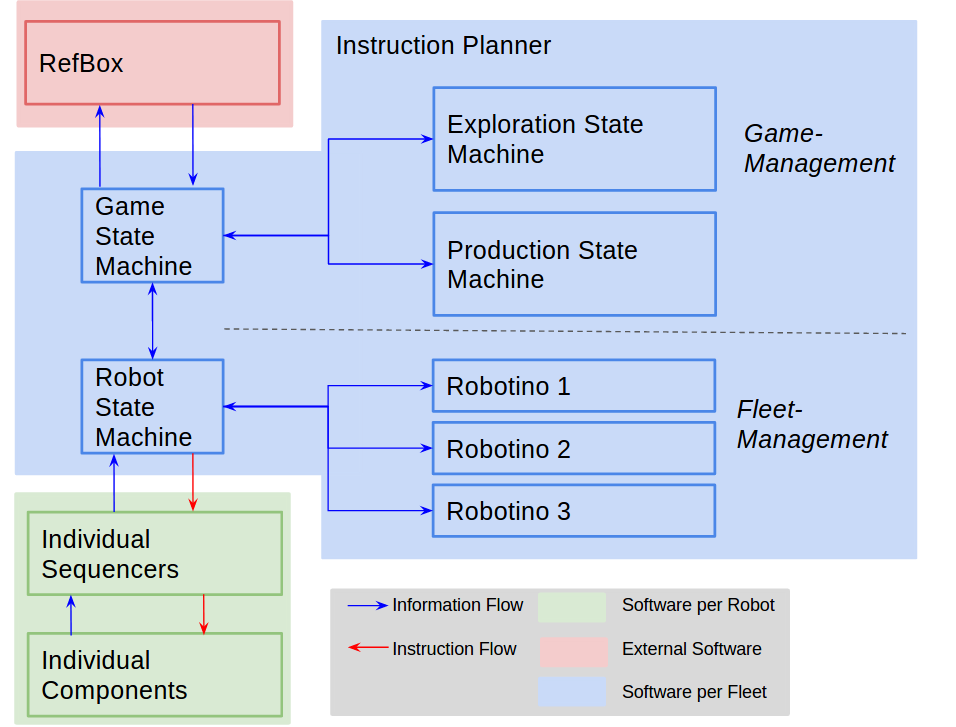
\includegraphics[scale=0.23]{pic/Instructionplanner2018.png}
\caption{Management of Robot Fleet and the Game Management}
\label{fig:instr_overview}
\end{figure}
\newpage

Since the blue-part of figure \ref{fig:instr_overview} handles the internal management, it can be treated as an agent that provides the next orders for the robots, based on their actual situation.\\
This situation is brought into the Instruction Planner via the Sequencers of each
robot.\\
In Green (once per robot): \\
\begin{itemize}
    \item \textbf{Sequencers}
    \begin{itemize}
        \item handle all events on robot
        \item local management of robot
    \end{itemize}
    \item \textbf{Components}
    \begin{itemize}
        \item provide skills
        \item get configurations and report via events
    \end{itemize}
\end{itemize}


\paragraph{Objective Management}
The objective management consists of multiple \textit{state machines}, that are in
a hierarchical order.
All state machines listen to the events that are received via the \textit{Sequencers}, or
the \textit{Refbox}.
The thought behind this architecture is an intelligent agent that can be "asked" for the next
best step to take.\\

\begin{itemize}
    \item \textbf{Game State Machine}
    \begin{itemize}
        \item first level state machine
        \item takes care of the game phases (e.g. Setup Phase, Exploration Phase, Production Phase)
         \item depending on the game state, events are forwarded to the next level state machine (e.g. Exploration State Machine)
    \end{itemize}
    \item \textbf{Exploration State Machine}
    \begin{itemize}
        \item takes care of all objectives that have to be fulfilled in the phase
        \item tells Sequencer, which position should be explored next
    \end{itemize}
\end{itemize}

\subsubsection{Changes}
Previously the purpose of the Instruction Planner was misunderstood, so the whole structure of this component had to be planned again. The implementation now differs a lot from the old one of 2017. Only view lines of code could be recycled and used again. A completely new system has been introduced: the \textit{hierarchical state machines}. The implementation of this system now is more modular, parts (e.g. the state machines for the phases) can easily be exchanged and replaced with other approaches or implementations. Overall the instruction planner has been completely redesigned and is still under construction.
%The previous implementation of the instruction planner as been changed completely to enhance the modularity.
%The now given Skeleton is designed to be easily extended in various ways, e.g. for the use of multiple Robots
%or the exchange of tactics using different implementation of agents. \\
%
%
%\begin{figure}[h]
%\centering
%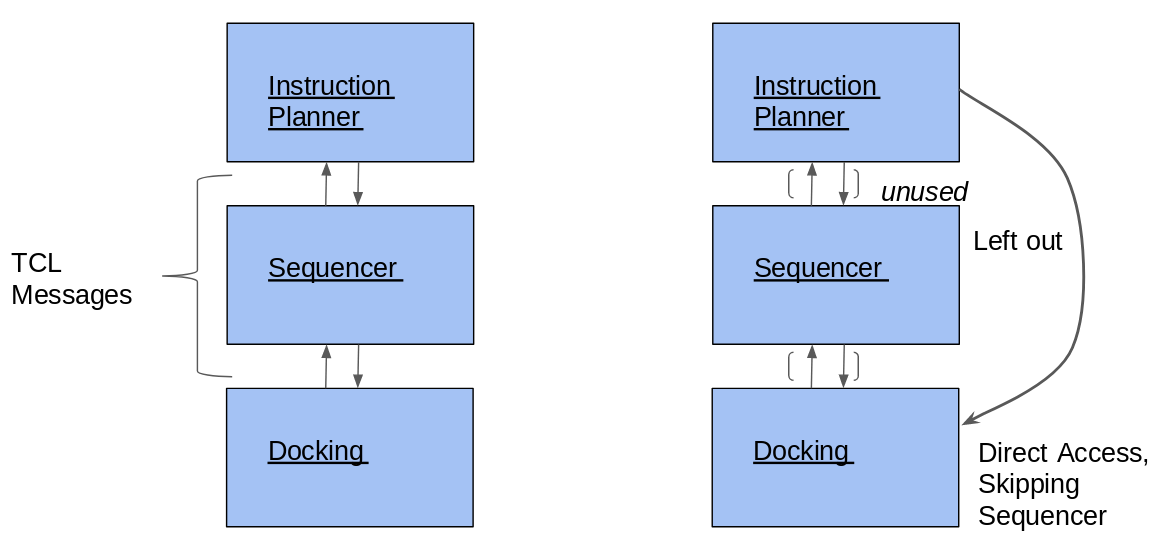
\includegraphics[scale=0.4]{pic/oldUse_Instructionplanner.png}
%\caption{design related changes in Instruction Planner and Sequencer}
%\label{fig:changes_instruction}
%\end{figure}
%
%The new version of the Instruction Planner does no longer work against the Smartsoft architecture\ref{fig:changes_instruction}.
%By changing the architecture as seen in the figure the complexity of the Instruction planner is reduced and the task distribution improved.\\

%The implementation now differs a lot from the old of 2017. Only view lines of code could be recycled and used again.
%A completely new system has been introduced: the \textit{hierarchical state machines}. The implementation of
%this system now is more modular, parts (e.g. the state machines for the phases) can easily be exchanged and
%replaced with other approaches or implementations. \\
%Overall the instruction planner has been completely redesigned and is still under construction.

\subsubsection{Conclusion}
With the new architecture of the Instruction Planner multiple new features can be implemented.
\begin{itemize}
    \item \textbf{Multiple Robots:} The new implementation would allow the use of multiple robots on the field, since
    the new architecture considers the use of multiple Sequencers.
    \item \textbf{Intelligent Agents:} The \textit{Objective Management} is designed to work with agents that can be asked
    for the next steps, in the actual case the implementation works with state machines. Other implementations of Agents can
    also fitted to the interface.
    \item \textbf{Divide and Conquer:} Separating the robot management from the objective management separates two problems
    that can be handled individually: \textit{Objective Manager} creates the next task and the \textit{Fleet Manager} takes care
    of all robots and assigns this task to the best candidate. For the Fleet Manager, a full concept is needed, which is not part of this report.
\end{itemize}

The actual level of production does not contain a fully functional Instruction Planner.
The current state consists of the skeleton of the parts. The implementation of the
actual agent is missing as well as the logic to distribute the tasks to multiple robots.
Probably, the first implementation of the \textit{Objective Manager} might be a
simple static implementation of a "following a pattern of points" approach in combination with a simple \textit{Fleet Manager} that
assigns just one order at a time to only one robot.
